\section{自由度答疑记录}

\subsection{虎克铰相关的问题}

可能大家对于一些简单机构的自由度还不是很熟悉。虎克铰本身也是一个比较容易让人迷惑的机构,重点是要明白虎克铰的构造。虎克铰的与球铰相比,其特点为保证链接的方向是任意的,但是不能产生扭转,两个虎克铰可以组成一个只能传递单向扭矩的万向传动装置。比如四个虎克铰组成的平行四边形,可能有一些人无法想象它是无法扭动的,建议想象成两组万向节(就是汽车传动轴)传动。这样就会发现一旦扭动,那么杆件自身就会产生扭转,这是与机构自身杆件不会扭转的假设矛盾的。想通了这个不会扭动的问题,可以对于PU*为什么只有空间中的三个平动自由度有更深的理解。

\begin{figure}[htb]
    \centering
    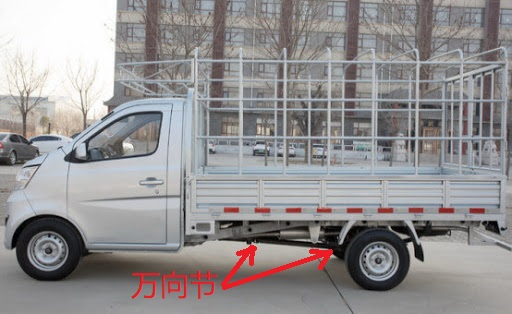
\includegraphics[width=.5\linewidth]{smalltruck.jpg}
    \caption{汽车上的万向节,可以观察身边的小货车}
\end{figure}

